\documentclass{article}
\usepackage[utf8]{inputenc}
\usepackage{graphicx}
\usepackage{listings}
\usepackage{amsmath}

\begin{document}
\title{os9}
\author{maryam bagherian}
\date{December 2020}
\maketitle
\section{Introduction}
\subsection{coffee}
Coffee is the most consumed beverage in the world after water.
Consuming the right amount of coffee a day prevents diseases such as stroke, cancer, Parkinson's disease, dementia and can reduce the risk of these diseases and health benefits such as increasing memory and concentration.
\subsection{image}
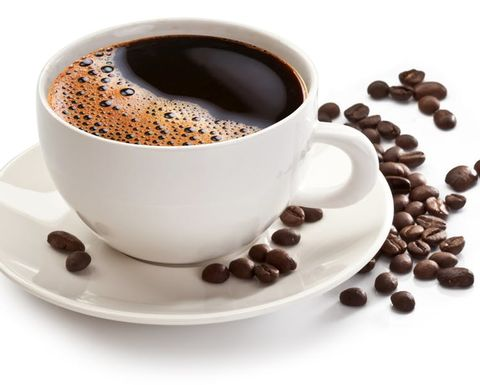
\includegraphics[width=10cm]{coffee.jpg}


\label{tab:table}
\begin{tabular}{|c|c|c|}
\hline
\textbf{Coffee drinks} & \textbf{Size in oz. (mL)} & \textbf{Caffeine (mg)}\\
\hline
Brewed & 8 (237) & 96 \\
Brewed,decaf & 8 (237) & 2\\
Espresso &  1 (30) & 64\\
Espresso, decaf & 1 (30) & 0\\
Instant  & 8 (237) & 62\\
Instant, decaf & 8 (237) & 2\\
\hline
\end{tabular}
\section{math formula}
\[
\sin^2(a)+\cos^2(a) = 1
\]
\section{Codes}
\begin{lstlisting}
#include<bits/stdc++.h>
using namespace std;
int achermann(int m, int n)
{
	if (m == 0)
		return (n + 1);
	if (m>0 && n == 0)
		return achermann(m - 1, 1);
	if (m>0 && n>0)
		return achermann(m - 1, achermann(m, n - 1));
}
int main()
{
	int a, b;
	cout << "enter 2 num:\n";
	cin >> a >> b;
	cout << "ANSWER:" << achermann(a, b);
	system("pause>n");
	return 0;
}
\end{lstlisting}
\end{document}
